\subsection{SRCNN}
Partimos del método descrito en \cite{SRCNN}, en el cual se menciona una red que cuente con al menos 3 capas convolucionales, de
manera que la primer capa se encargue de extraer los parches de baja resolución, la(s) capa(s) intermedias realizan el mapeo entre
los parches de baja resolución y los de alta resolución, y la última capa realizará la reconstrucción de la imagen de alta
resolución. Para ello hicimos uso de la libreria \textbf{keras} y de \textbf{tensorflow}.\\
\subsubsection{Entrenamiento de la red}
Para poder tener una SRCNN funcional, tuvimos que entrenar nuestro modelo a fin de lograr obtener los resultados que esperabamos.
Para este proceso de entrenamiento es necesario que en nuestro \emph{dataset} tengamos la imagen en alta resolución y su
correspondiente par de baja resolución. Para obtener las imagenes en baja resolución, se puede seguir el siguiente procedimiento:
\begin{enumerate}
    \item Reducir la escala de la imagen original (Alt resolución), puede ser en un factor de 2 o el que se desee.
    \item Reescalar la imagen que acabamos de reducir, dependiendo del factor de reducción de escala que hayamos utilizados, de
    manera que tengamos una imagen del mismo tamaño que la imagen de alta resolución. El resultado será una imagen que se verá
    borrosa, es decir, habremos reducido su resolución.
\end{enumerate}
Debido a esta forma de generar las imagenes de baja resolución, fue necesario tener un módelo SRCNN para cada factor de escalamiento
de imagen. Para nuestro caso se realizaron entrenamientos para 2 factores de escalamiento: \textbf{1)} Factor de 2 y \textbf{2)}
factor de 4.\\
Tambien fue necesario tomar en cuenta el espacio de color en el cual se realizará el entrenamiento, ya que de este depende la
\emph{forma} de la imagen de entrada de la red neuronal. Para nuestro casó realizamos modelos SRCNN para los espacios de color
\textbf{RGB} y \textbf{$YC_rC_b$}, de este úlitmo unicamente se toma como entrada el canal $Y$.\\

%%%%%%%%%%%%%%%%%%%%%%%%%%%%%%%%%% Texto que se podria utilizar en la sección de "discusiones" %%%%%%%%%%%%%%%%%%%%%%%%%%%%%%%%%%
\begin{comment}
Para el caso del espacio de color $YC_rC_b$ realizamos el entrenamiento únicamente en el
canal $Y$, ya que es en este canal en donde se concentra la mayor parte de la información de la imagen referente a los detalles y
texturas (Si vemos este canal por separado, sería como ver la imagen en escala de grises). Para el caso del espacio de color $RGB$
el entrenamiento fue realizado sobre los 3 canales, ya que en este espacio de color, los detalles y texturas de la imagen se
distribuyen entre los 3 canales.\\
\end{comment}
%%%%%%%%%%%%%%%%%%%%%%%%%%%%%%%%%%%%%%%%%%%%%%%%%%%%%%%%%%%%%%%%%%%%%%%%%%%%%%%%%%%%%%%%%%%%%%%%%%%%%%%%%%%%%%%%%%%%%%%%%%%%%%%%%

Los diseños de la red neuronal convolucional tienen la siguiente estructura:
\begin{table}[H]
    \centering
    \caption{Red convolucional para espacio de color $YC_rC_b$}
    \begin{tabular}{|l|l|l|l|l|}
    \hline
    \textbf{Capa} & \textbf{Filtros} & \textbf{Kernel}  & \textbf{Inicializador de Kernel} & \textbf{Función de activación}\\ \hline
    1             & 128              & $9\times9$       & \emph{Glorot\_Uniform}           & ReLU                 \\
    2             & 64               & $5\times5$       & \emph{Glorot\_Uniform}           & ReLU                 \\
    3             & 1                & $5\times5$       & \emph{Glorot\_Uniform}           & Lineal               \\ \hline
    \end{tabular}
\end{table}

\begin{table}[H]
    \centering
    \caption{Red convolucional para espacio de color $RGB$}
    \begin{tabular}{|l|l|l|l|l|}
    \hline
    \textbf{Capa} & \textbf{Filtros} & \textbf{Kernel}  & \textbf{Inicializador de Kernel} & \textbf{Función de activación}\\ \hline
    1             & 128              & $9\times9$       & \emph{Glorot\_Uniform}           & ReLU                 \\
    2             & 64               & $5\times5$       & \emph{Glorot\_Uniform}           & ReLU                 \\
    3             & 3                & $5\times5$       & \emph{Glorot\_Uniform}           & Lineal               \\ \hline
    \end{tabular}
\end{table}

En cuanto al optimizador se utilizaron los siguientes valores de parámetros:

\begin{table}[H]
    \centering
    \caption{Parámetros de entrenamiento del optimizador \textbf{Adam}}
    \begin{tabular}{|l|l|l|l|l|l|}
    \hline
    \textbf{Capa} & \textbf{$\beta_1$} & \textbf{$\beta_2$}  & \textbf{$\alpha$ menor a 150 epocas} & \textbf{$\alpha$ mayor o igual a 150 epocas} & \textbf{$\epsilon$}\\ \hline
    1             & 0.9           & 0.999          & 0.003                                        & 0.001                                        & 1e-9                 \\
    2             & 0.9           & 0.999          & 0.003                                        & 0.001                                        & 1e-9                 \\
    3             & 0.9           & 0.999          & 0.0003                                       & 0.0001                                       & 1e-9                 \\ \hline
    \end{tabular}
\end{table}

Se utilizó un \emph{dataset} de 91 imagenes para el entrenamiento de todos los modelos desarrollados y la métrica utilizada fue el
error cuadrático medio (MSE).

%%%%%%%%%%%%%%%%%%%%%%%%%%%%%%%%%%%%% Entrenamiento del módelo RGB con factor de escalamiento de 4 %%%%%%%%%%%%%%%%%%%%%%%%%%%%%%
\subsubsection{Entrenamiento del modelo SRCNN: RGB con factor de escalamiento 4}
Previo al entrenamiento de este módelo fue necesario \emph{normalizar} la imagen, por lo cual primero se divide la imagen entre
255, dado que se entrena sobre los 3 canales $RGB$ y recordemos que el espacio de color RGB puede tomar valores en el intervalo
$[0-255]$ por cada canal. El \emph{normalizado} de la imagen se realiza con el fin de que la red varíe su salida en un intervalo
de $[0-1]$, de esta forma \emph{reducimos} la variación de los parámetros de la red.\\
Este módelo fue entrenado hasta 2525 epocas, donde cada epoca representa un recorrido completo a todo el dataset, es decir, un
entrenamiento con todas las 91 imagenes que tiene el dataset. En la imagen \ref{fig:SRCNN_MSE_TrainingLoss4RGB} se muestran
los resultados del entrenamiento de la red desde la epoca 2475 hasta la epoca 2525.

\begin{figure}[H]
    \centering
    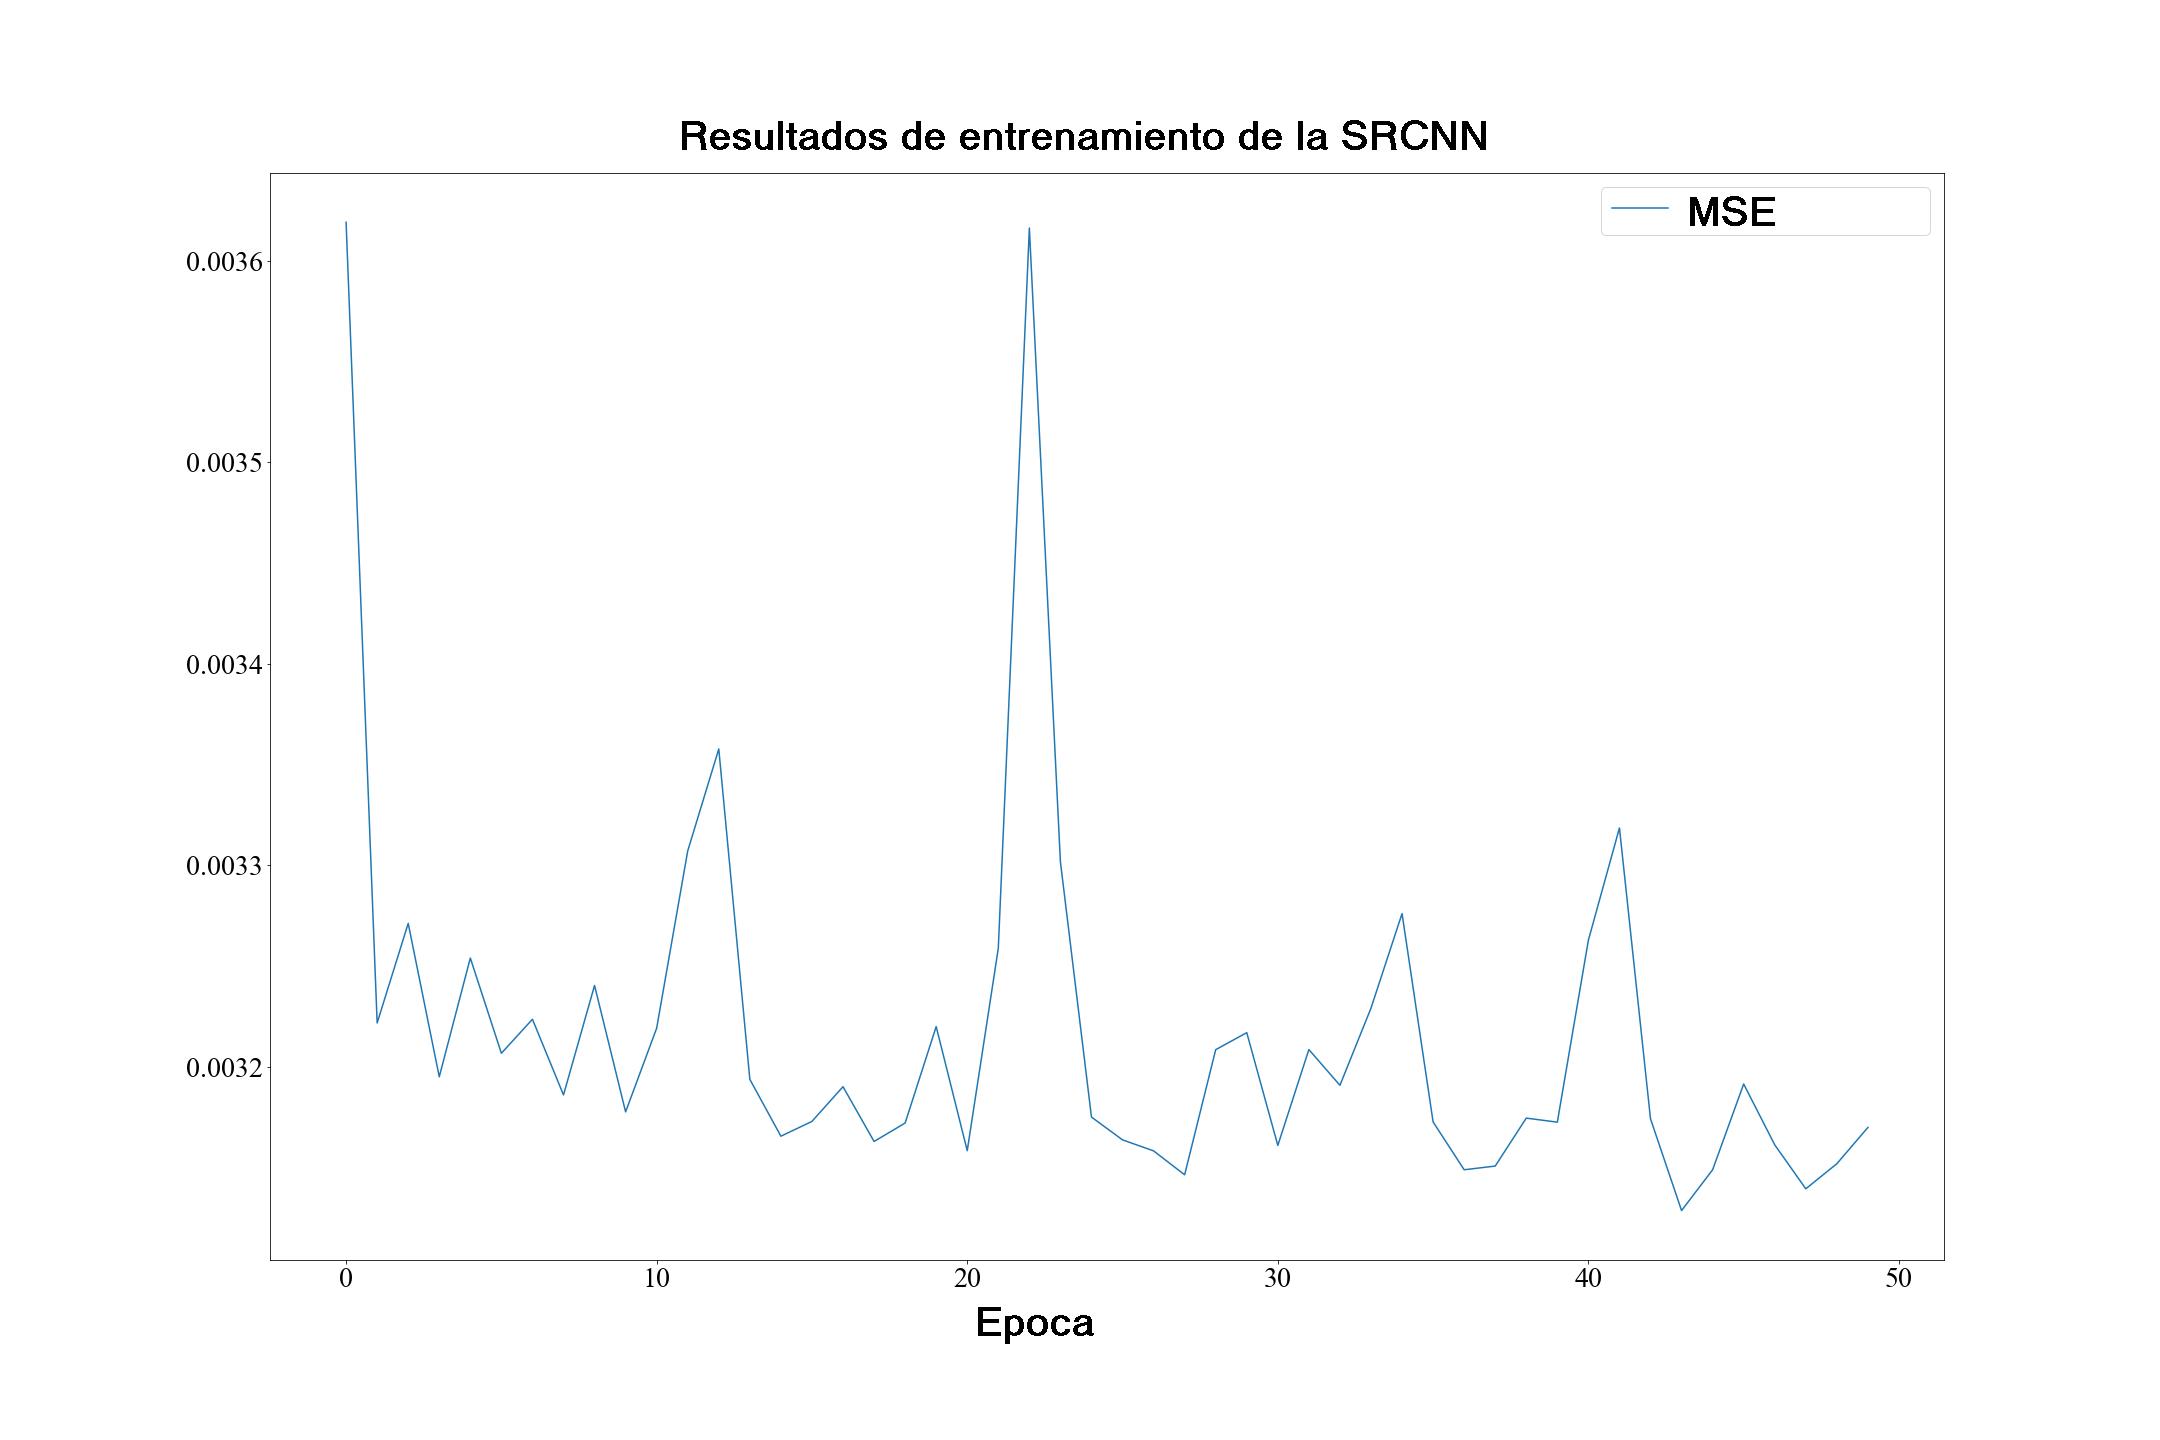
\includegraphics[scale=0.35]{TrainingHistory_2475-2525_epochs_4RGB.png}
    \caption{Minimización de función de costo (MSE) de red convolucional RGB con factor de escalamiento 4}
    \label{fig:SRCNN_MSE_TrainingLoss4RGB}
\end{figure}

Cabe mencionar que esto fue un re-entrenamiento de la red, es decir, partimos del módelo que ya teniamos generado hasta las 2475
epocas y desde ese punto comenzamos el nuevo entrenamiento de la red. Los resultados de entrenamiento previos a los resultados
que se observan en la figura \ref{fig:SRCNN_MSE_TrainingLoss4RGB} no se muestran en este documento, ya que la información que
proporcionan no resulta muy legible. En la figura \ref{fig:SRCNN_MSE_TrainingProcess4RGB} se observa gradualmente el proceso de
entrenamiento de la red conforme transcurría la epoca $i$ de entrenamiento.

\begin{figure}[H]
    \centering
    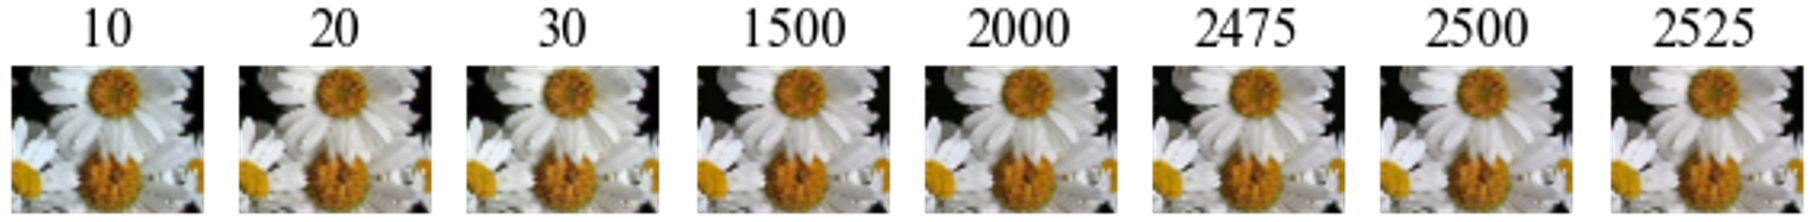
\includegraphics[scale=0.45]{ProcesoEntrenamiento_RGB4.png}
    \caption{Proceso de aprendizaje de la red convolucional RGB con factor de escalamiento de 4}
    \label{fig:SRCNN_MSE_TrainingProcess4RGB}
\end{figure}

%%%%%%%%%%%%%%%%%%%%%%%%%%%%%%%%%%%%% Entrenamiento del módelo RGB con factor de escalamiento de 2 %%%%%%%%%%%%%%%%%%%%%%%%%%%%%%
\subsubsection{Entrenamiento del modelo SRCNN: RGB con factor de escalamiento 2}
Se realizó, de igual manera que en el caso anterior, un normalizado de la imagen a modo de \emph{pre-procesamiento} de imagen.
Este módelo fue entrenado desde 0 hasta 350 epocas. En la imagen \ref{fig:SRCNN_MSE_TrainingLoss2RGB} se muestran los resultados
del entrenamiento de la red durante las primeras 200 epocas.

\begin{figure}[H]
    \centering
    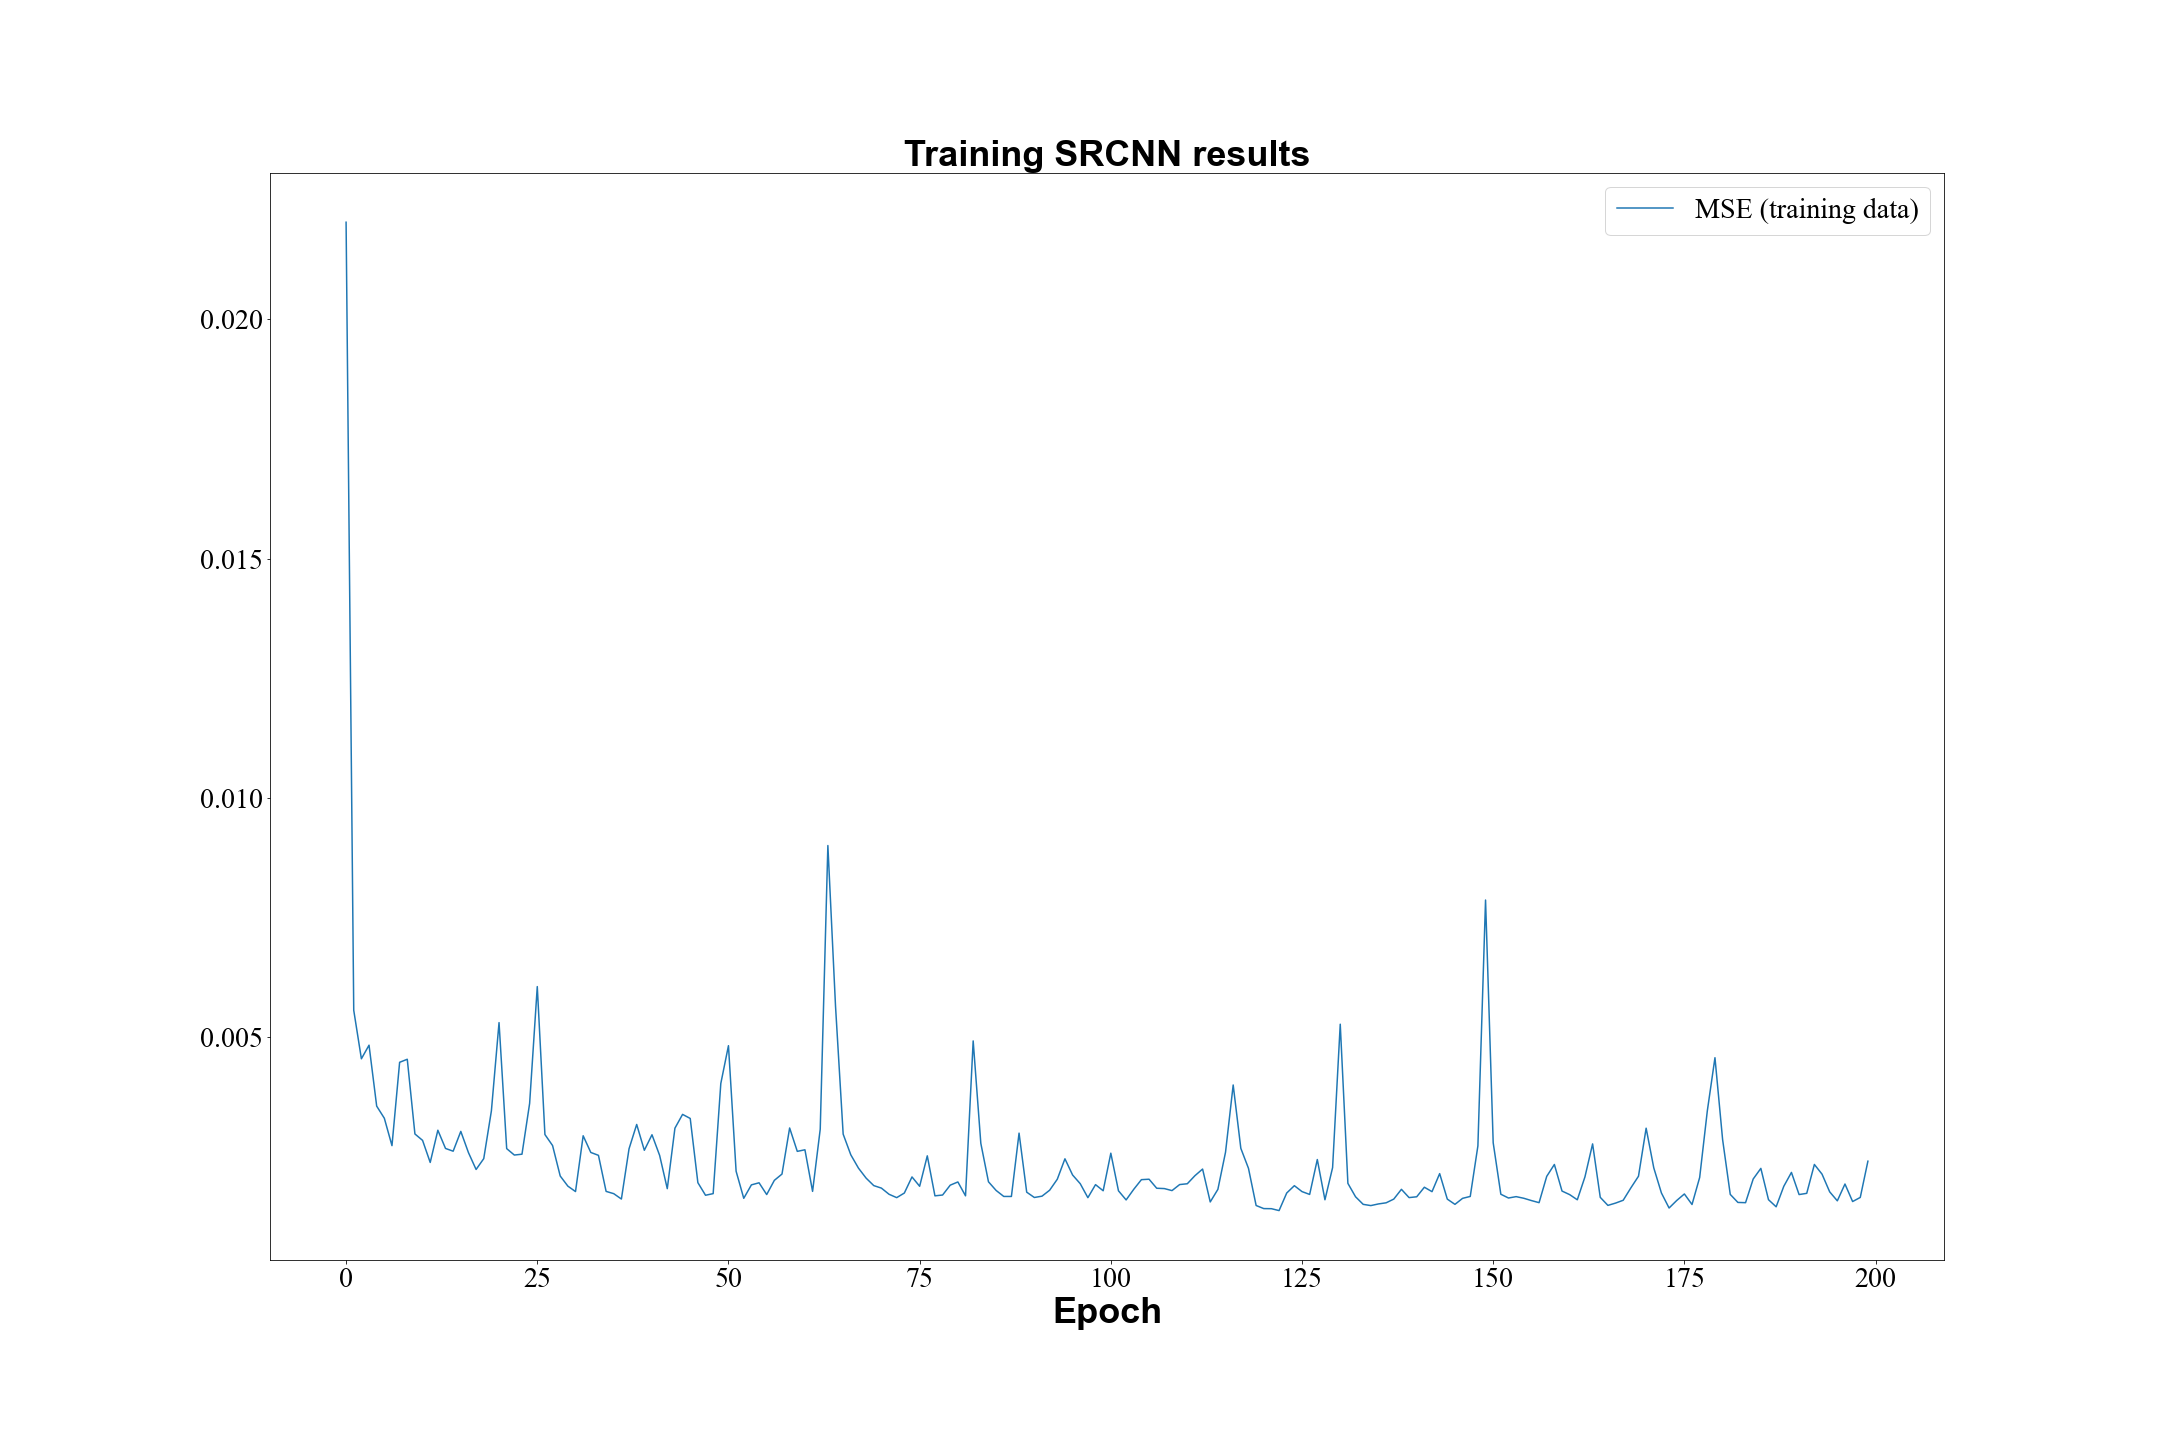
\includegraphics[scale=0.25]{TrainingHistory_0-200_epochs_2RGB.png}
    \caption{Minimización de función de costo (MSE) de red convolucional RGB con factor de escalamiento 2}
    \label{fig:SRCNN_MSE_TrainingLoss2RGB}
\end{figure}

A diferencia del caso anterior, este módelo fue entrenado menor cantidad de epocas, por lo que los resultados que se observan
 en la figura \ref{fig:SRCNN_MSE_TrainingLoss2RGB} se pueden leer de manera más adecuada. En la figura
 \ref{fig:SRCNN_MSE_TrainingProcess2RGB} se observa gradualmente el proceso de entrenamiento de la red conforme transcurría la
 epoca $i$ de entrenamiento.

\begin{figure}[H]
    \centering
    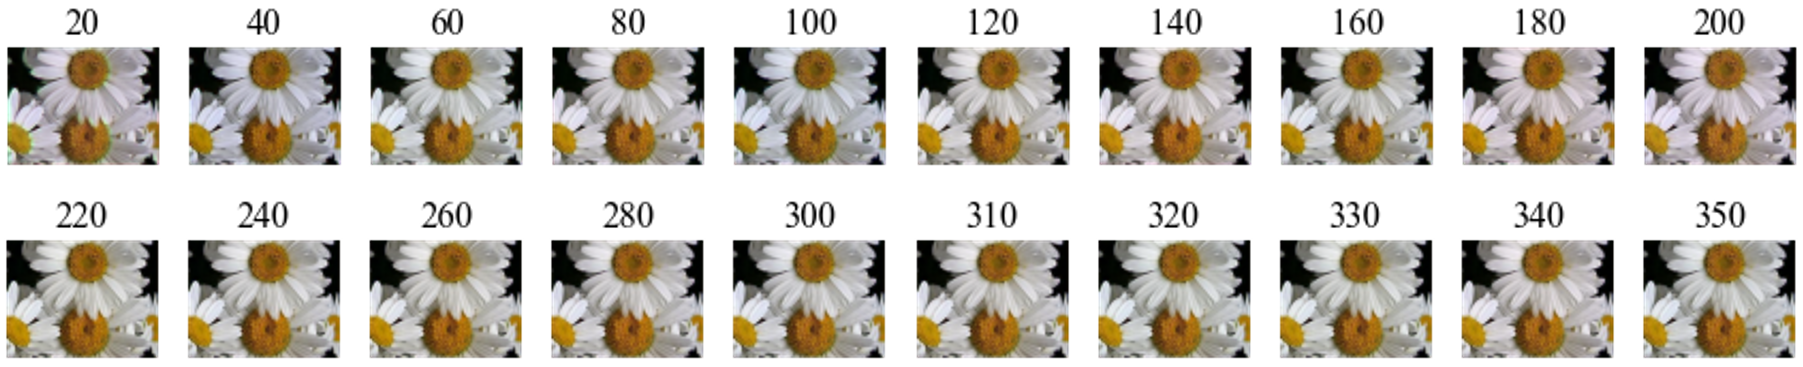
\includegraphics[scale=0.45]{ProcesoEntrenamiento_RGB2.png}
    \caption{Proceso de aprendizaje de la red convolucional RGB con factor de escalamiento de 2}
    \label{fig:SRCNN_MSE_TrainingProcess2RGB}
\end{figure}

%%%%%%%%%%%%%%%%%%%%%%%%%%%%%%%%%%%%% Entrenamiento del módelo YCrCb con factor de escalamiento de 4 %%%%%%%%%%%%%%%%%%%%%%%%%%%%%%
\subsubsection{Entrenamiento del modelo SRCNN: $YC_rC_b$ con factor de escalamiento 4}
Fue mencionado anteriormente en este documento, que, cuando se entrena el módelo en el espacio de color $YC_rC_b$, únicamente se
maneja el canal $Y$ de este espacio de color. Por lo que debemos realizar un pre-procesamiento de la imagen de la siguiente manera:
\begin{enumerate}
    \item Convertimos del espacio de color $RGB$ a $YC_rC_b$ pero sin haber normalizado la imagen RGB, es decir, con sus valores en el rango $[0-255]$
    \item Normalizamos esta imagen convertida. Para ello dividimos la imagen entre 255, y esta imagen será la entrada a nuestra red.
\end{enumerate}
Este módelo fue entrenado desde 0 hasta 250 epocas. En las siguientes figuras respectivamente se muestran los resultados del
entrenamiento de la red desde 0 a 200 epocas y después un \emph{re-entrenamiento} de 200 a 250 epocas.

\begin{figure}[H]
    \centering
    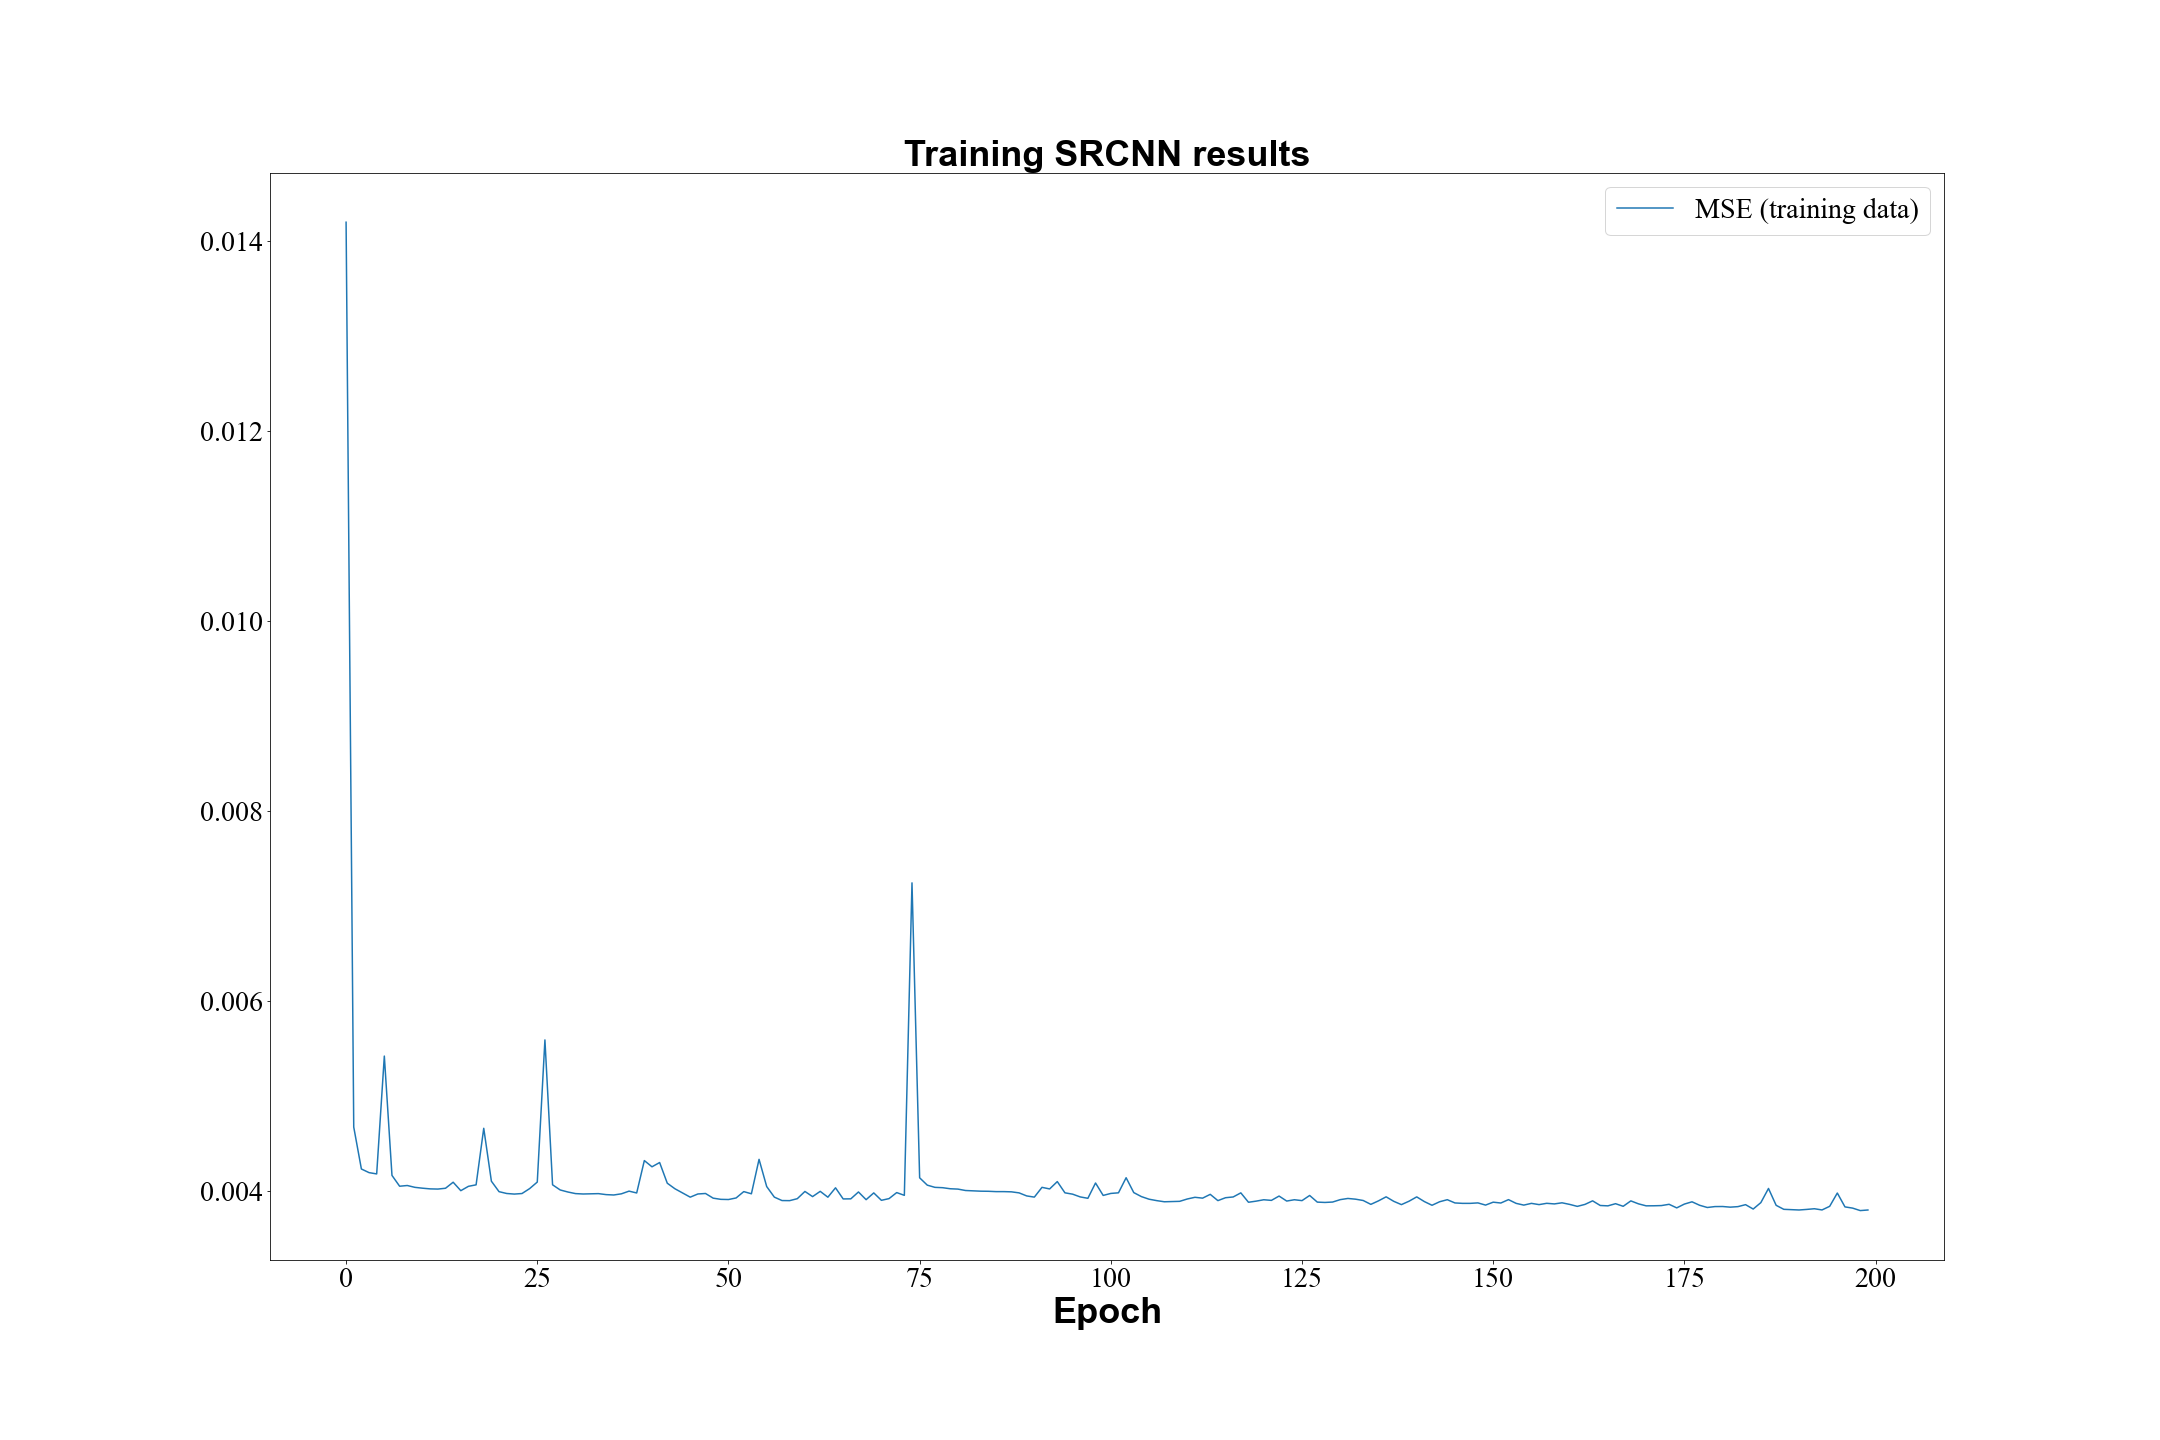
\includegraphics[scale=0.15]{TrainingHistory_0-200_epochs_4Y.png}
    \caption{Minimización de función de costo (MSE) de red convolucional $YC_rC_b$ con factor de escalamiento 4}
    \label{fig:SRCNN_MSE_TrainingLoss4Y1}
\end{figure}

\begin{figure}[H]
    \centering
    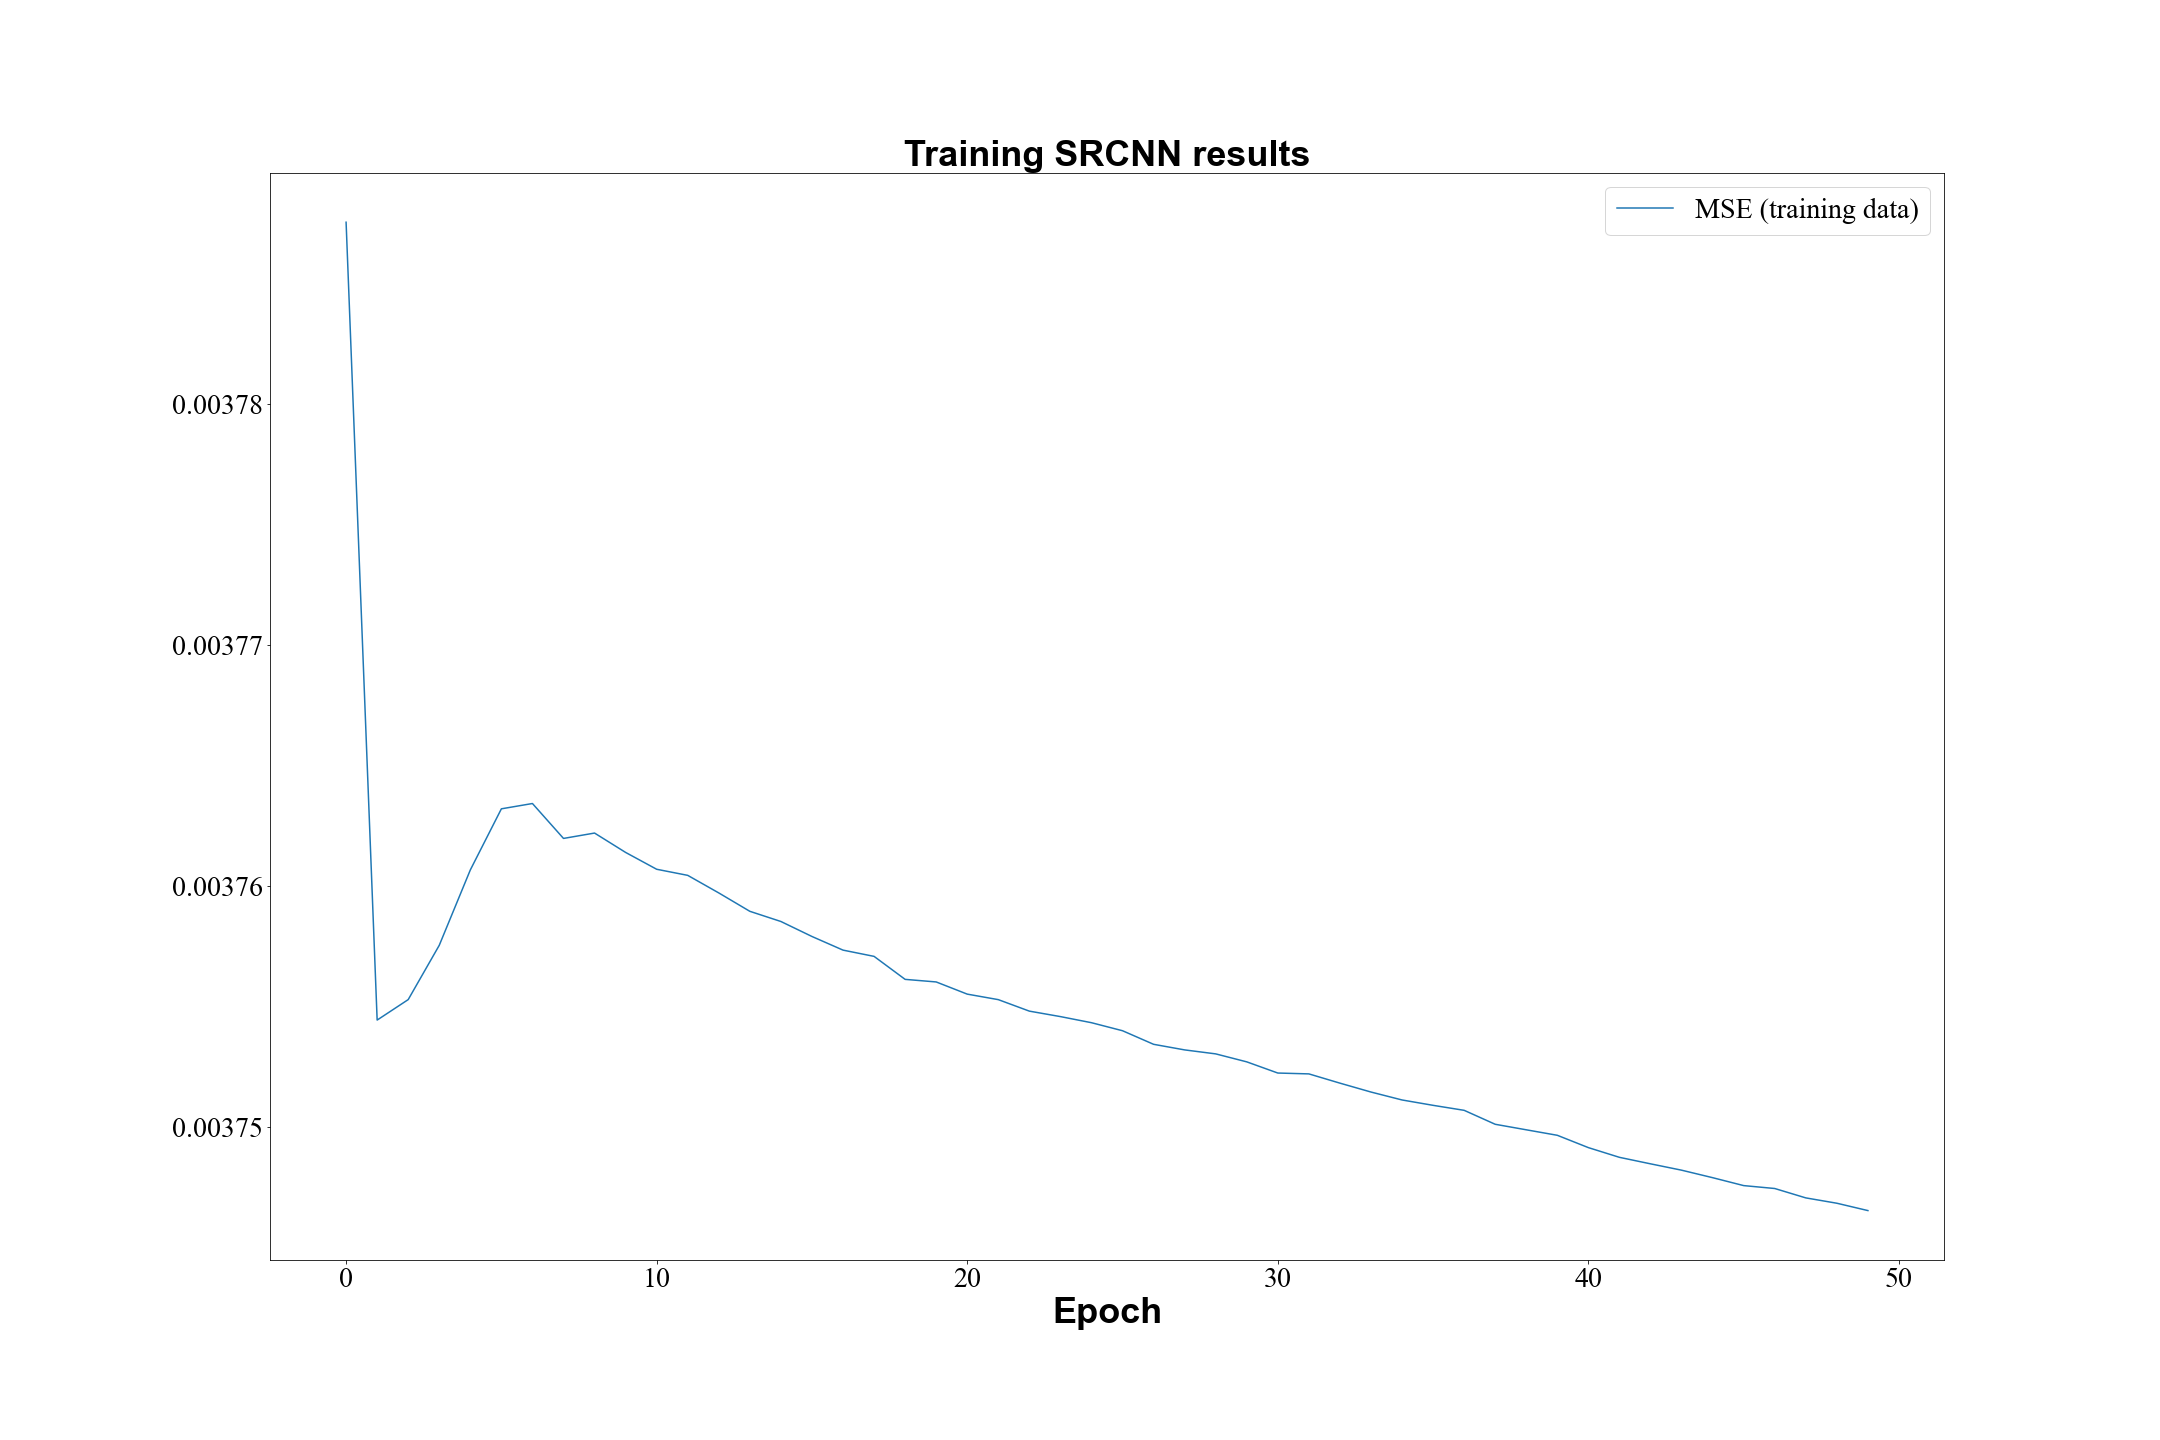
\includegraphics[scale=0.15]{TrainingHistory_200-250_epochs_4Y.png}
    \caption{Minimización de función de costo (MSE) de red convolucional $YC_rC_b$ con factor de escalamiento 4}
    \label{fig:SRCNN_MSE_TrainingLoss4Y2}
\end{figure}

En la figura \ref{fig:SRCNN_MSE_TrainingProcess4Y} se observa gradualmente el proceso de entrenamiento de la red conforme
transcurría la epoca $i$ de entrenamiento.

\begin{figure}[H]
    \centering
    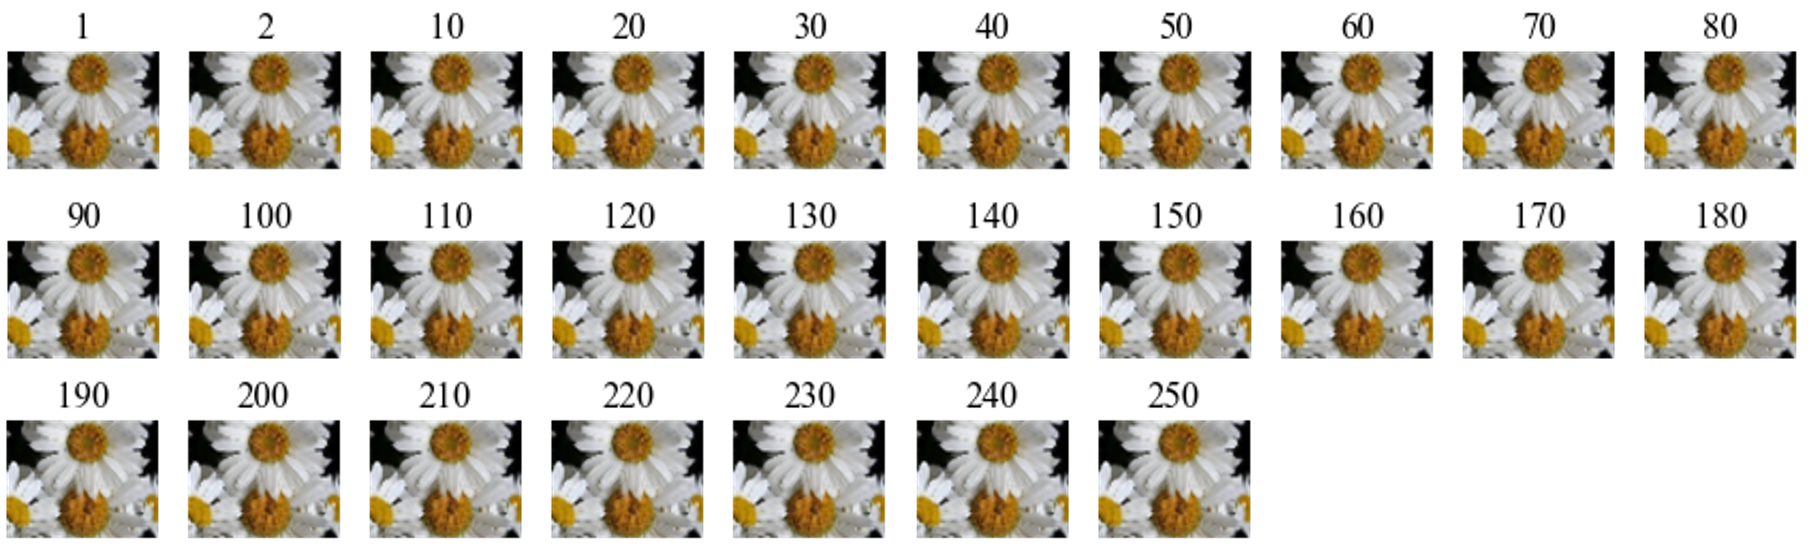
\includegraphics[scale=0.45]{ProcesoEntrenamiento_Y4.png}
    \caption{Proceso de aprendizaje de la red convolucional $YC_rC_b$ con factor de escalamiento de 4}
    \label{fig:SRCNN_MSE_TrainingProcess4Y}
\end{figure}

%%%%%%%%%%%%%%%%%%%%%%%%%%%%%%%%%%%%% Entrenamiento del módelo YCrCb con factor de escalamiento de 2 %%%%%%%%%%%%%%%%%%%%%%%%%%%%%%
\subsubsection{Entrenamiento del modelo SRCNN: $YC_rC_b$ con factor de escalamiento 2}
Se realiza el mismo procedimiento que en el caso anterior para \emph{pre-procesar} la imagen.
Este módelo fue entrenado desde 0 hasta 250 epocas. En las siguiente figura \ref{fig:SRCNN_MSE_TrainingLoss2Y} se muestran los
resultados del entrenamiento de la red.

\begin{figure}[H]
    \centering
    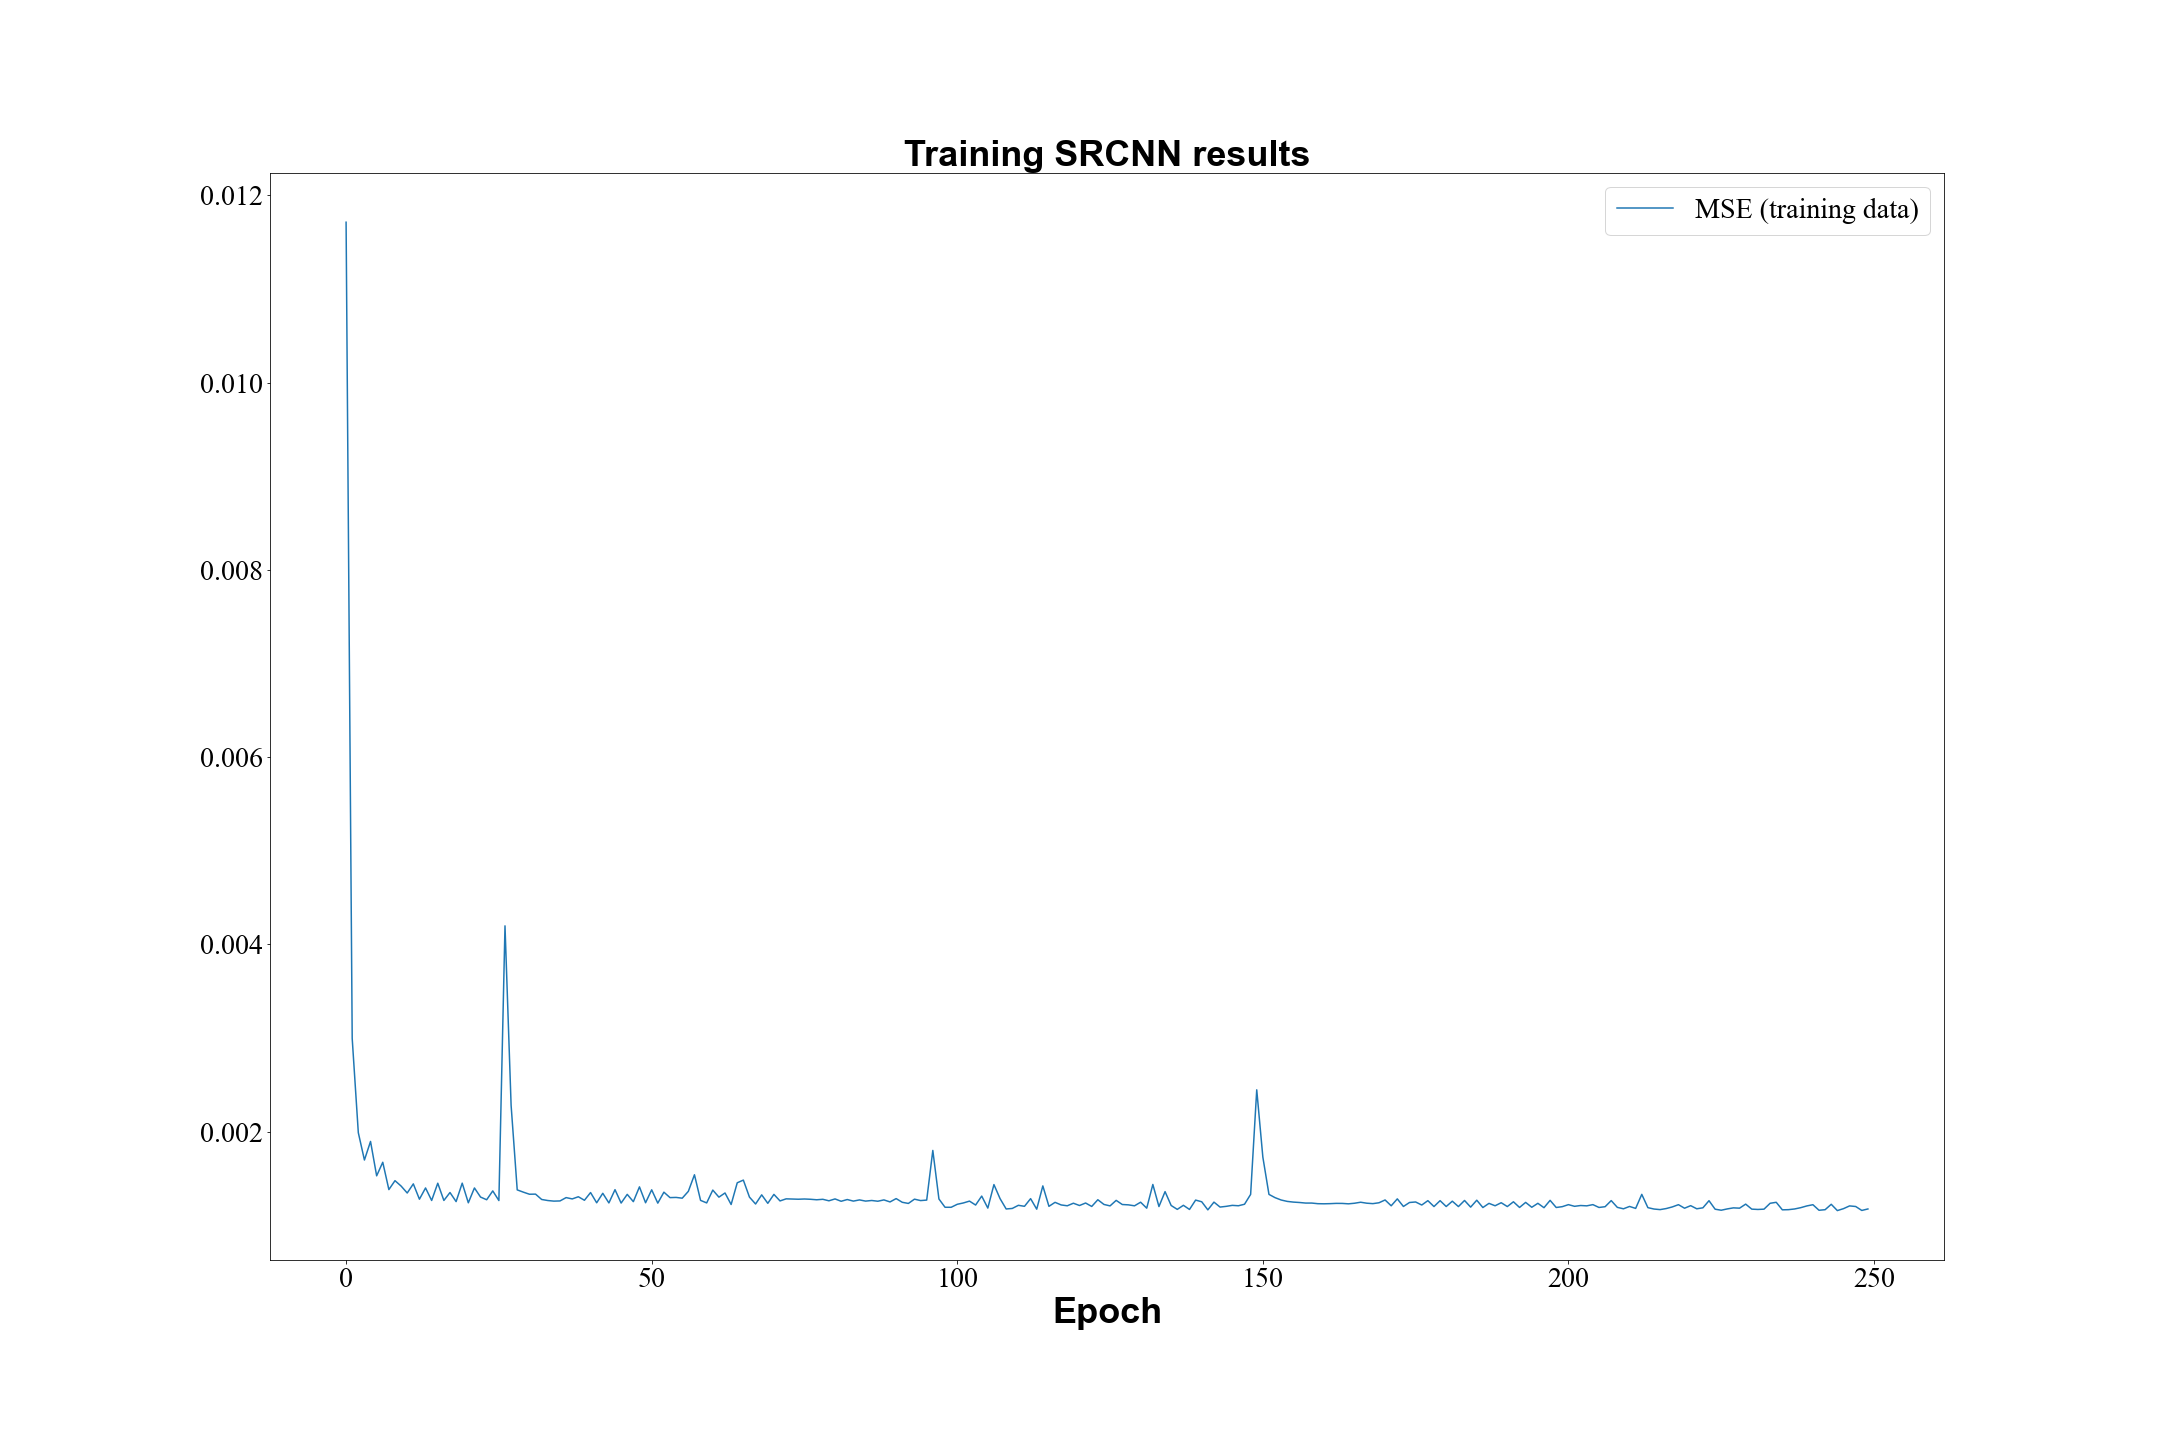
\includegraphics[scale=0.15]{TrainingHistory_0-250_epochs_2Y.png}
    \caption{Minimización de función de costo (MSE) de red convolucional $YC_rC_b$ con factor de escalamiento 2}
    \label{fig:SRCNN_MSE_TrainingLoss2Y}
\end{figure}

En la figura \ref{fig:SRCNN_MSE_TrainingProcess2Y} se observa gradualmente el proceso de entrenamiento de la red conforme
transcurría la epoca $i$ de entrenamiento.

\begin{figure}[H]
    \centering
    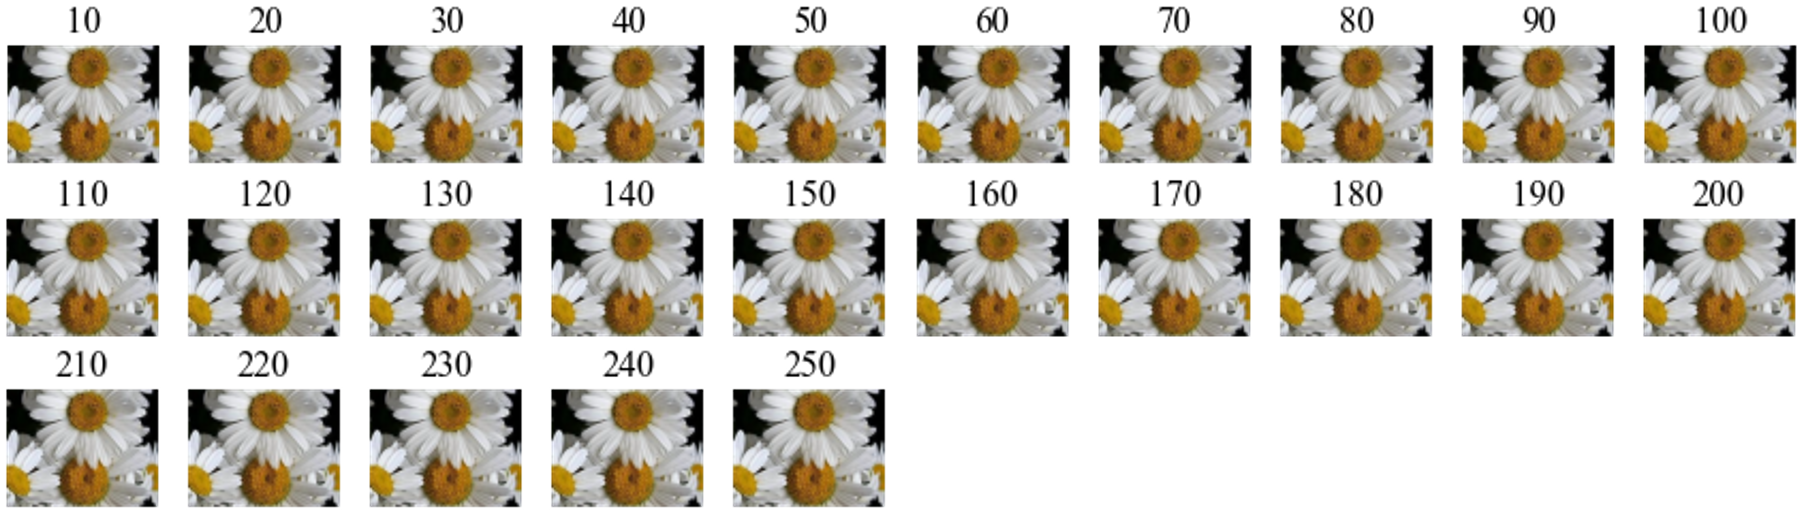
\includegraphics[scale=0.45]{ProcesoEntrenamiento_Y2.png}
    \caption{Proceso de aprendizaje de la red convolucional $YC_rC_b$ con factor de escalamiento de 2}
    \label{fig:SRCNN_MSE_TrainingProcess2Y}
\end{figure}